\section{HTML5 para o desenvolvimento de jogos casuais}

Nesse capítulo serão abordadas as ferramentas mais utilizadas para
desenvolvimento de jogos casuais dentro do ambiente HTML5.
As ferramentas atuais que suportam HTML5 possuem muitas vantagens,
principalmente em portabilidade, tirando do desenvolvedor a
responsabilidade de implementação de código para várias plataformas, mas
com isso também introduz algumas limitações para que o jogo
desenvolvido possa funcionar em vários dispositivos e sistemas
operacionais. Esse capítulo visa mostrar as vantagens e desvantagens
de cada uma das ferramentas utilizadas no HTML5, o que pode ser usado
com tranquilidade e o que necessita de mais cautela no seu uso.

\subsection{Javascript como ferramenta}

Como dito no capítulo anterior, Javascript é a principal ferramenta
quando se vai trabalhar em um jogo com HTML5, pois é ela que vai
manipular as propriedades dos elementos para passar ao jogador a
impressão de movimento do protagonista do jogo.
Javascript é uma linguagem muito poderosa que suporta vários tipos de
sintaxes, e possui muitas vantagens de uma linguagem de alto nível,
como por exemplo coletor de lixo (garbage collector), e tipagem
dinâmica, o que ajuda o desenvolvedor a se preocupar menos com tipos
de variáveis e elementos, e evita a grande preocupação com o
gerenciamento de memória.
Como desvantagem, o Javascript tende a expor o código do jogo em
questão para a internet, pois para que um navegador execute o jogo é
necessário que o mesmo possua o código, tendo em vista que Javascript
não é uma linguagem compilada, e sim interpretada. Uma das técnicas
utilizadas para evitar a distribuição do código para o usuário é a
ofuscação de código. Com essa técnica o seu código continua chegando
ao usuário, mas de uma maneira não legível, ou seja, será facilmente
entendida pelo navegador mas dificilmente entendida por um humano que
quer utilizar seu código-fonte.
Uma das grandes preocupações de todos os desenvolvedores de jogos é a
performance. A área de jogos exige muito processamento para calcular
cada um dos passos que um jogador vai dar dentro de um jogo, como cada
objeto vai se comportar, calcular trajetórias de projéteis, calcular
iluminação dos objetos da cena, calcular a física dos objetos e outras
coisas, e para isso é necessário utilizar muito processamento do
dispositivo que estiver executando o mesmo.
Sabe-se que o código Javascript será interpretado em cima de um navegador, que por sua vez está sendo
executado pelo sistema operacional e dividindo memória e processamento
com outros programas no escalonador de processos, portanto não
é possível esperar que um jogo que vai rodar no navegador tenha as mesmas
capacidades que um jogo que executa nativamente no sistema
operacional, com código compilado para a própria plataforma.
Sabendo a média de performance que é exigida por um jogo,
deve-se em consideração que um jogo casual que utiliza apenas
coisas simples, como física básica, calculo de trajetórias e
movimentação de imagens é totalmente aceitável para ser executado em
dispositivos que possuem baixa performance, desde que bem executado.

\subsection{Navegadores como plataforma}

Os navegadores são a parte fundamental para a execução do jogo, pois
ele é a plataforma de desenvolvimento que o desenvolvedor está visando,
ou seja, assim como muitas grandes empresas visam vídeo games,
computadores ou celulares como plataforma-alvo de desenvolvimento, o
desenvolvedor deve ter em mente que está desenvolvendo para o
navegador, e estar ciente de suas vantagens, desvantagens e
limitações.

Um dos grandes problemas de se trabalhar com navegadores é a
fragmentação, pois o desenvolvedor deve pensar em quais navegadores e
dispositivos o seu jogo estará disponível, levando em consideração
que cada usuário vai escolher seu navegador preferido, e que talvez
esse navegador não estará na ultima versão. Atualmente vários sites na
internet descrevem quais funcionalidades do HTML5 estão disponíveis em
qual navegador, um deles é o dive into html5 que está disponível
online em \citeonline{website:diveintohtml5}.
Esse problema acontece também no desenvolvimento para computadores e
vídeo games, mas é um pouco mais simples de lidar, pois os jogos
simplesmente não são compatíveis, ou seja, se você tem um computador
que o hardware não é bom o suficiente para executar um jogo, ele será
barrado já na instalação, ou será executado mas será impossível de ser
jogado devido a sua lentidão. O mesmo acontece com os jogos no
navegador, caso o navegador não tenha suporte às funcionalidades que o
jogo precisa, ele provavelmente não será executado. Enquanto o
desenvolvimento do jogo estiver sendo feito, o desenvolvedor deve ter
definido quais são as plataformas alvo do seu jogo, pois apesar de
estar lidando com navegadores que podem executar em uma grande
quantidade de plataformas, é nítido que não será possível ter a mesma
performance em todas elas, tendo em vista que um computador pessoal
possui muito mais capacidade de processamento do que um celular, por
exemplo.

O problema da fragmentação pode ser mais facilmente contornado quando
o desenvolvedor fixa algumas configurações, como por exemplo a versão
dos navegadores suportados. A liberdade do desenvolvedor é total,
bastando apenas ter em mente o quanto de processamento será utilizado
e quais funcionalidades serão necessárias para a execução do jogo.

\subsection{Canvas}

O Canvas provê uma interface com resolução de dependências para
desenhar coisas diretamente no navegador, e pode ser utilizado para
gerar gráficos, gráficos de jogos, e outras imagens para serem
visualizadas no momento da execução. \cite{website:w3ccanvas}.

O canvas na web segue a mesma interface que é utilizada nas grandes
plataformas atuais. O conceito de canvas foi criado pela Apple para
utilizar no webkit do MacOS X. \cite{lubbers2010pro}. Com essa
funcionalidade foi crianda uma API
para desenhar widgets e outras coisas em sua plataforma, e essa API
vem sendo padronizada e implementada em vários navegadores.

Essa tecnologia é fundamental para o desenvolvimento de jogos para
o navegador, pois permite ao desenvolvedor uma forma de exibir
objetos e manipulá-los da mesma forma que é feito com jogos
simples em duas dimensões para computadores.
Diferentemente do DOM, que cria vários objetos que podem ser
manipulados individualmente pelo navegador, o canvas quando criado
gera apenas um elemento no navegador, e todos os elementos criados
nesse elemento (imagens, retângulos e etc) ficam invisíveis para acesso, e
não podem ser modificados, apenas recriados.

O canvas pode ser utilizado em várias camadas, gerando vários
elementos canvas dentro do navegador, e posicionando-os no mesmo
lugar, facilitando a manipulação de cenário e melhorando a
performance.

Na Figura~\ref{img:angrybirds}, é mostrado um exemplo do jogo Angry
Birds, que utiliza canvas com várias camadas para a renderização padrão.

\newlength{\imgwidth}
\setlength{\imgwidth}{16.09cm}
\newlength{\imgheight}
\setlength{\imgheight}{10.59cm}

\begin{figure}[H]
  \centering
	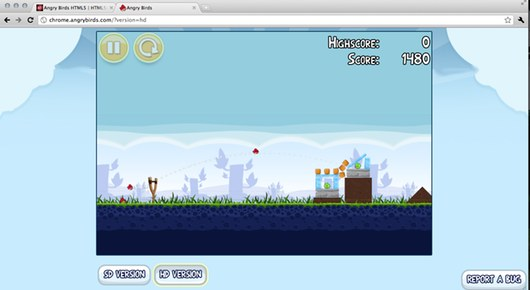
\includegraphics[height=\imgheight,width=\imgwidth]{angrybirds}
  \caption{Angry Birds {--} utilizando canvas em varias camadas}
  \label{img:angrybirds}
\end{figure}


\subsection{Transformações e transições com CSS3}

O CSS3 possui uma série de transformações e transições que permitem o
desenvolvedor rotacionar e escalar os elementos de uma página
\cite{agi2011html5}. Apesar da grande movimentação dos desenvolvedores
em função do desenvolvimento de jogos utilizando as funcionalidades do
Canvas, muito ainda é discutido sobre utilizar DOM para o
desenvolvimento de jogos, assim aproveitando as vantagens que o CSS3
pode trazer.
Uma das vantagens de ter um jogo que utiliza DOM ao invés de Canvas é
a maior compatibilidade com os navegadores, pois todos possuem suporte
a DOM, que é utilizado para a renderização das páginas de internet que
estão funcionando atualmente.

O CSS3 foi criado para suprir as necessidades de criações de efeitos
visuais para páginas de internet comuns, dando aos elementos DOM a
possibilidade de se transformar de várias maneiras. Ao ver essa nova
gama de funcionalidades algumas pesquisas foram feitas pelos
desenvolvedores para saber quais eram as vantagens de utiliza-las para
o desenvolvimento de jogos para o navegador.

As transições e transformações do CSS3 são muito úteis ao utilizar
objetos DOM para um jogo pois todos esses efeitos são renderizados
pelo navegador com aceleração de hardware, com isso ganhando
performance com os efeitos visuais.

\subsection{SVG}

SVG é uma linguagem de marcação utilizada para descrever aplicações de gráficos
bi-dimensionais e imagens, e um conjunto de scripts relacionados a
interfaces gráficas. \cite{website:w3csvg}. Essa linguagem é utilizada por
editores como o Inkscape para definir os vetores criados por ele.

Comparando SVG com Canvas, é possível verificar uma grande diferença
em termos de desenho. SVG é utilizado para construir desenhos
vetoriais que podem ser facilmente modificados, diferentemente do
canvas, que possui uma particularidade de não poder ser alterado, ou
seja, após um objeto canvas ser desenhado ele não pode ser mais
modificado, apenas redesenhado.

Com SVG também é possível fazer animações, assim possibilitando a
criação de mídias mais interativas, como logotipos animados e pequenas
animações de introdução.

Na Figura~\ref{img:timetrap}, é possível ver o logo da empresa
Timetrap, que foi desenvolvido apenas com SVG, utilizando animações. O
logo animado pode ser visto em
http://files.myopera.com/emoller/blog/timetrap.html conforme
\citeonline{website:svgtimetrap}.

\begin{figure}[H]
  \centering
	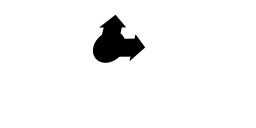
\includegraphics[height=\imgheight,width=\imgwidth]{timetrap}
  \caption{Logo da empresa Timetrap {--} Utilizando apenas vetores SVG para sua construção}
  \label{img:timetrap}
\end{figure}

No desenvolvimento de jogos a utilização do SVG é bem limitada, sendo
comumente utilizada para as animações acima citadas. O motivo do SVG
não ser utilizado para o desenho dos jogos é a dificuldade e
performance de alterar cada um dos vetores, por esse motivo
a técnica de sprites é mais utilizada, favorecendo imagens pré-feitas
ao invés da manipulação de vetores.


\subsection{WebSocket API}

WebSocket API define uma especificação que permite as páginas web
utilizar o protocolo de Sockets para fazer comunicação em duas
vias com um servidor remoto. \cite{website:w3cwebsockets}. Com essa tecnologia
conseguimos facilmente criar jogos multiplayer, pois podemos
trocar informações entre dois computadores de uma maneira bem mais
veloz, trafegando menos dados e recebendo as informações mais
rapidamente.
O que traz essa velocidade na comunicação via internet é não utilizar
o método normal de comunicação que o HTTP fornece, e sim utilizar um
túnel direto entre o computador e o servidor.
Nos métodos normais de comunicação utilizando o HTTP a cada requisição
é necessário passar por todo o processo de comunicação do TCP, e
receber todos os dados e metadados do HTTP, o que gera um tempo maior para
o recebimento dos dados e um maior tráfego de rede. Com o Socket (que
é criado pela funcionalidade de WebSockets), apenas uma conexão TCP é
criada e mantida durante um período de tempo, assim facilitando o
tráfego de informações, viabilizando uma comunicação mais rápida e
usável para um jogo em tempo real.

Websockets possibilita uma redução de 500 para 1 ou até 1000 para 1
(em alguns casos) de cabeçalhos de HTTP desnecessários, e até 3 para 1
em latência. \cite{lubbers2010pro}.

Na Figura~\ref{img:swarmation}, é apresentado um jogo que utiliza
uma biblioteca que disponibiliza uma interface de código WebSockets,
a finalidade dela é tentar manter as mesmas interfaces em
todos os navegadores, inclusive os que não possuem suporte para essa
tecnologia.

A ideia do jogo é integrar vários jogadores em um único lugar, sendo que
cada jogador assume o papel de um pixel, e eles precisam formar uma
determinada imagem que é gerada aleatoriamente pelo jogo e mostrada à
direita. A função do WebSockets nesse jogo é sincronizar em tempo real a
posição de cada jogador para que ao final da contagem saber quais imagens
foram formadas e quais jogadores devem ser pontuados.

\begin{figure}[H]
  \centering
	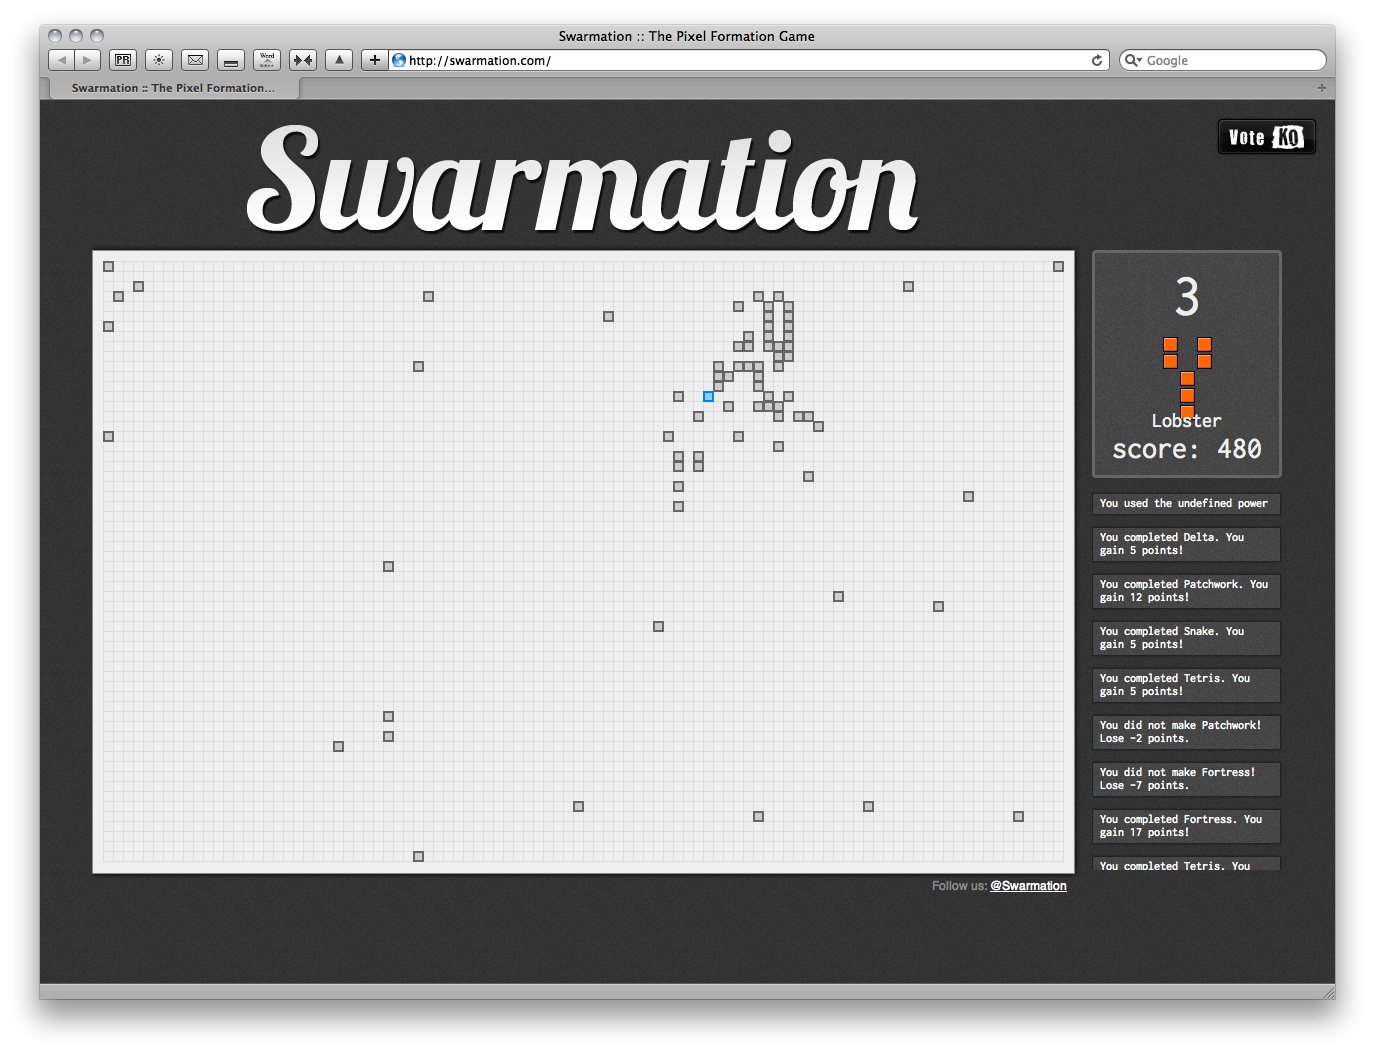
\includegraphics[height=\imgheight,width=\imgwidth]{swarmation}
  \caption{Swarmation {--} Jogo casual simples que utiliza Websockets}
  \label{img:swarmation}
\end{figure}


\subsection{Offline cache}

Offline cache, em sua maneira mais simplista, é uma lista apontando
para o HTML, CSS, Javascript, imagens e outros recursos que devem
estar disponíveis para o website. \cite{pilgrim2010html5}. O arquivo de
manifesto é o responsável por conter essa lista de arquivos, provendo
ao navegador a informação sobre os recursos que
precisam ser utilizados quando o dispositivo que está executando a
página em questão não estiver apto a acessar a internet, ou seja,
na primeira requisição, tudo que estiver disponível no arquivo de manifesto
que contem essa lista será baixado, guardado no dispositivo e utilizado até
que o manifesto seja modificado.

A cada nova requisição de uma aplicação que utiliza offline cache o
navegador verifica o arquivo de manifesto se ele não foi modificado
o navegador vai utilizar os arquivos que estão disponíveis localmente,
caso contrário todos os arquivos da seção "CACHE" desse arquivo serão baixados novamente.

A funcionalidade de offline cache também prevê as requisições que não
podem ser guardadas localmente, requisições que precisam
necessariamente estar online para funcionar corretamente, e para isso
existe uma seção chamara REMOTE no arquivo manifesto, definindo quais
são os arquivos que não devem ser considerados quando o usuário não
estiver offline.

Todos os arquivos utilizados na aplicação devem estar no arquivo de
manifesto para os arquivos que não estarão disponíveis localmente há
uma seção chamada FALLBACK.

Utilizando Offline cache é possível criar uma aplicação para a
internet que funcione normalmente sem a necessidade do usuário estar
conectado. Um exemplo dessa funcionalidade foi feito na aplicação da
Figura~\ref{img:currency}. A aplicação em questão pode ser adicionada
no celular como um favorito (no caso do iPhone, pode ser adicionado
como um novo aplicativo à tela principal do aparelho) e ser utilizada
normalmente como se fosse uma aplicação nativa.

\begin{figure}[H]
  \centering
	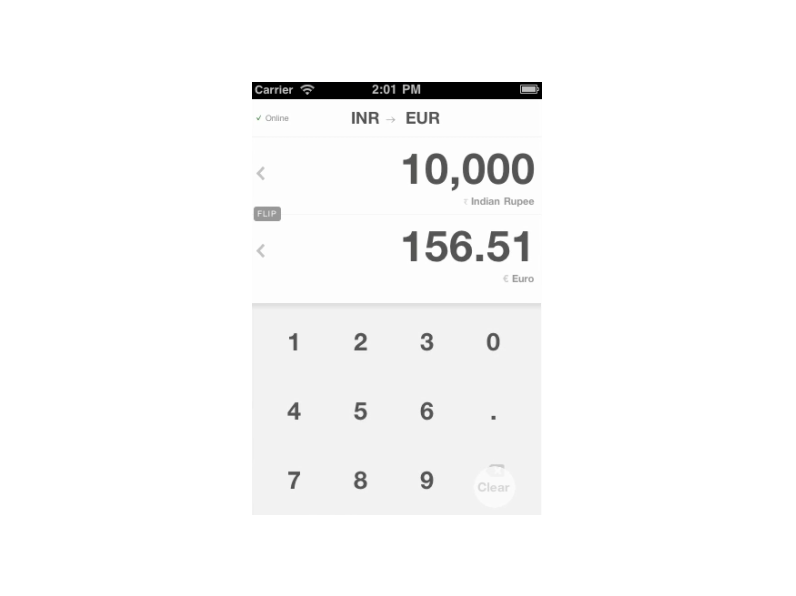
\includegraphics[height=\imgheight,width=\imgwidth]{currency}
  \caption{Offline cache {--} Currency.io utilizando offline cache
  para fazer uma aplicação que ficará disponível mesmo sem acesso a
  internet.}
  \label{img:currency}
\end{figure}

Essa funcionalidade pode ser muito utilizada em jogos casuais para disponibilizar um
determinado para utilização em um dispositivo móvel, bastando
adicionar o jogo aos favoritos, e ele estará disponível a qualquer
momento.


\subsection{Local Storage}

Local Storage do HTML5 provê aos websites uma maneira de guardar
informações e recuperá-las depois, utilizando um conceito similar aos
cookies, mas já pensando em um grande modelo de dados. \cite{pilgrim2010html5}.
Por muito tempo os desenvolvedores utilizaram cookies para guardar
informações sobre o website diretamente no navegador do usuário, e
essa tecnologia se provou muito ineficiente para uma quantidade um
pouco maior de dados, pois além de ser limitado para guardar informações,
os dados ficam trafegando pela rede em cada requisição, consumindo
banda, expondo os dados, e deixando as requisições mais lentas.

O Local storage foi criado para resolver esses problemas, dando uma
interface simples para o desenvolvedor guardar dados de sua
aplicação diretamente no navegador do usuário. Para guardar tais dados
o desenvolvedor utiliza um banco que armazena dados seguindo um
esquema chave-valor, ou seja, uma chave como índice, associado a um
determinado valor, que será convertido para texto quando adicionado.

Essa funcionalidade é muito utilizada em conjunto com a funcionalidade
de offline cache, pois quando uma aplicação não possui conexão com a
internet é necessário utilizar Local Storage para guardar informações
que serão sincronizadas com o servidor assim que a aplicação possuir
conexão com a internet novamente.

Um exemplo que ilustra muito bem a utilização de local storage é a
aplicação do Google para visualização do Gmail offline (vide
figura~\ref{img:gmailoffline}), que utiliza local storage para guardar
as informações dos emails que ele controla, e utiliza offline cache
para manter a aplicação disponível sem a necessidade de conexão com a
internet.

\begin{figure}[H]
  \centering
	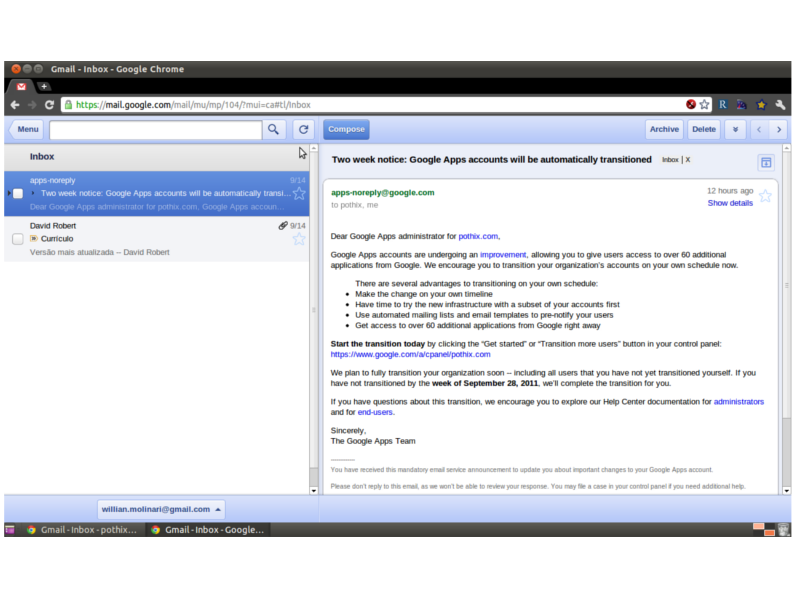
\includegraphics[height=\imgheight,width=\imgwidth]{gmailoffline}
  \caption{Offline cache {--} Currency.io utilizando offline cache
  para fazer uma aplicação que ficará disponível mesmo sem acesso a
  internet.}
  \label{img:gmailoffline}
\end{figure}

Utilizando essas funcionalidades para jogos casuais, é possível
guardar informações de tabelas de pontos, nomes dos jogadores,
informações sobre os níveis e falas dos personagens durante o jogo e
etc. Quando a funcionalidade de offline cache for utilizada, local
storage provavelmente será utilizada em conjunto para manter a
consistência dos dados do jogador, e possibilitar uma possível
sincronização com um servidor externo assim que houver conexão com a
internet.

\subsection{Áudio}
A uma das funcionalidades construídas para suprir uma das necessidades multimídia
da internet foi a \tagaudio. Com o passar do tempo e o aumento no
numero de sites, os conteúdos da internet foram mudando
e se tornando cada vez mais multimídia, e não apenas hipertexto de
acordo com a ideia inicial. Para utilizar esse tipo de mídia na
internet foram utilizados componentes externos, como o Adobe Flash por
exemplo, pois a internet ainda não estava preparada para resolver esse
tipo de problema.

O padrão HTML5 define uma forma para adicionar áudio a uma página de
internet de uma maneira fácil e sem depender de produtos externos.
Isso é feito através da \tagaudio, que traz uma
implementação nativa (que será feita pelos navegadores) para que o
áudio seja executado.

Essa funcionalidade fornece uma API Javascript para a manipulação do
áudio inserido no documento conforme \citeonline{pfeiffer2010definitive},
com isso é possível parar, pausar, tocar,
pular entre várias partes do áudio, entre outras funcionalidades.

Um dos problemas que podem ser encontrados com a \tagaudio é o tipo de
implementação de formatos que cada navegador suporta. Há um exemplo
simples desse problema na atual data de escrita desse trabalho. O
navegador Firefox possui a implementação do formato \textit{ogg}, que
é um formato aberto, enquanto outros navegadores como o Chrome por
exemplo, implementam o formato \textit{mp3}. Esse problema pode ser
facilmente contornado pela implementação atual da \tagaudio,
apenas definindo os dois formatos na mesma tag permitindo que o
navegador escolha o arquivo correto para ser executado.

A \tagaudio possui algumas particularidades que não permitem uma
resposta rápida e pode atrapalhar a jogabilidade provendo um som com
atraso. Para resolver esse problema está sendo desenvolvido a
Web audio API, que fornece APIs bem parecidas com a \tagaudio, mas
tratando os eventos no momento certo, lidando com a taxa de
atualização de cada dispositivo.

\begin{figure}[H]
  \centering
	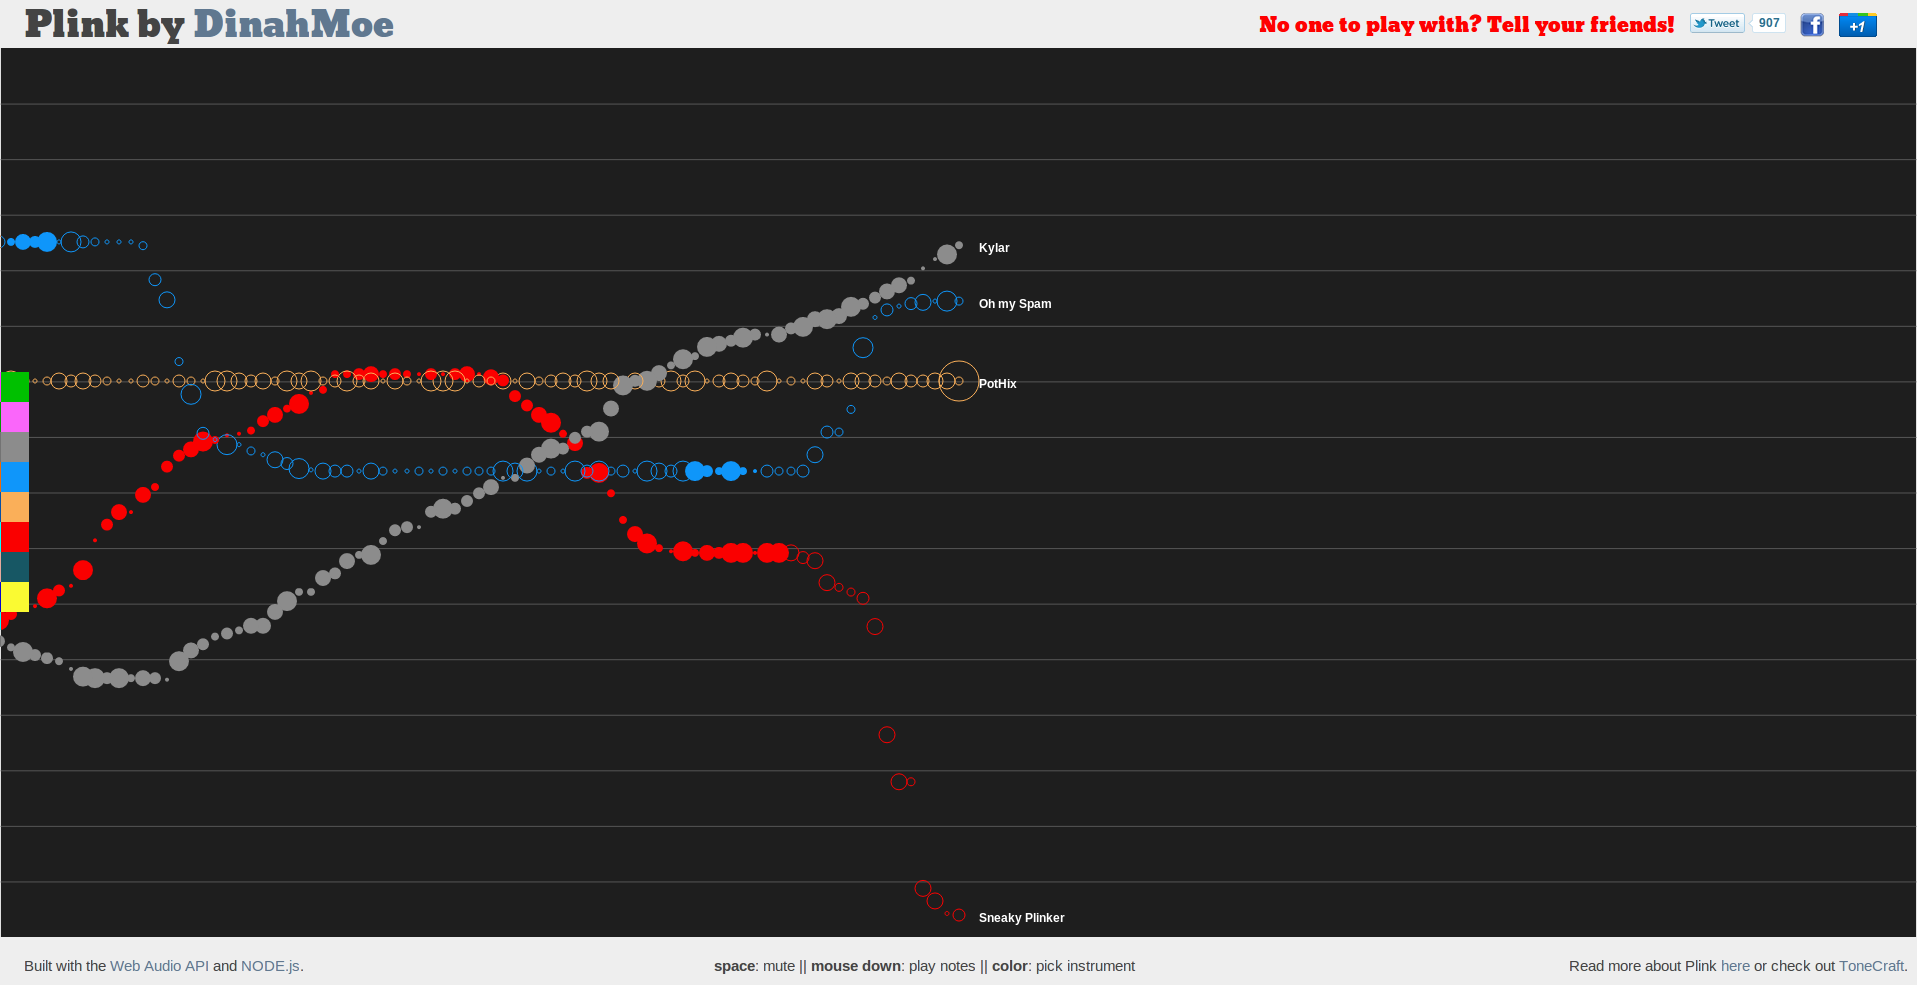
\includegraphics[height=\imgheight,width=\imgwidth]{webaudioapi}
  \caption{Plink {--} Jogo feito utilizando Web Audio Api}
  \label{img:webaudioapi}
\end{figure}

A figura~\ref{img:webaudioapi} mostra o jogo Plink, que utiliza Web
Audio Api para fornecer aos usuários uma forma divertida de interagir
entre si e criar musicas. Cada usuário controla sua posição com o
mouse, e o som gerado depende da sua posição e cor. Esse é um ótimo
exemplo de como a Web Audio Api está trazendo a manipulação de audio
em tempo real para o navegador, assim resolvendo os problemas de
latencia da tag audio.

Essas funcionalidades são muito úteis para o desenvolvimento de jogos, pois
todos os sons que o jogo deve produzir podem ser adicionados e
manipulados utilizando essas funcionalidades, assim criando uma
experiencia mais divertida para o jogador.

\subsection{WebGL}

Seguindo a definição de \cite{lubbers2010pro}, WebGL é uma API para gráficos 3D na web. Essa
API possibilita a criação de jogos que exigem mais processamento pelo
computador pois utiliza a GPU do dispositivo em questão para processar
os gráficos do jogo.

Essa tecnologia é baseada no OpenGL ES2, apenas um mapeamento para
Javascript conforme \citeonline{lubbers2010pro}, portanto possui
quase todas as funcionalidades que as versões para celular possuem,
inclusive shaders. Essa particularidade contribui
para que os atuais desenvolvedores de jogos (principalmente jogos em
três dimensões) tenham mais facilidade para portar os jogos mais
simples para web, apenas lidando com as particularidades de cada
navegador e com o fluxo diferenciado que um jogo web terá.

O WebGL é baseado na tag canvas, e utiliza a mesma tag utilizada para
se fazer desenhos canvas comums, mas ao invés de utilizar o contexto
2D, é utilizado o contexto 3D.

Um dos possíveis problemas de se utilizar WebGL na atual data desse
de escrita desse trabalho é a falta de suporte dos navegadores e
dispositivos para essa funcionalidade. Como o WebGL depende muito do
hardware do dispositivo, dar suporte para ele ainda é um problema,
pois depende dos drivers de cada dispositivo funcionar
corretamente, além do navegador possuir suporte para o mesmo.
WebGL está sendo bem utilizado atualmente para acelerar a execução do jogo,
mas não depender totalmente dele para que o jogo funcione, assim
aproveitando as vantagens do WebGL para os navegadores e sistemas que
possuem esse suporte.

Na figura~\ref{img:webglmodels} é possível ver modelos 3D no formato
MD2 (o mesmo formato que o jogo Quake II utilizava para seus
personagens) utilizando WebGL para a renderização. Isso é feito utilizando a
biblioteca GLGE, que é um facilitador para a utilização do WebGL.

\begin{figure}[H]
  \centering
	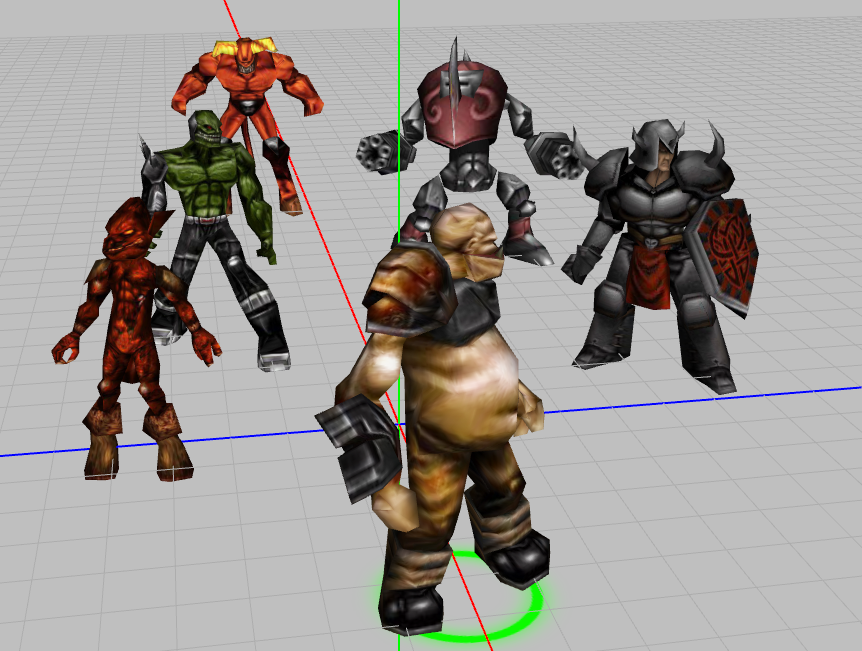
\includegraphics[height=\imgheight,width=\imgwidth]{webglmodels}
  \caption{Modelos 3D {--} Modelos de personagens 3D sendo renderizados com WebGL}
  \label{img:webglmodels}
\end{figure}

A figura~\ref{img:webglmodels} dá uma ideia de para onde o WebGL está
caminhando, e provavelmente daqui a algum tempo será possível criar
jogos 3D simples que funcionarão diretamente no navegador, ou seja, há
possibilidade que os jogos simples em três dimensões que estão atualmente
disponíveis para celulares serem desenvolvidos novamente para que
sejam executados diretamente no navegador num futuro não tão distante.

Outro exemplo de como WebGL pode ser poderoso pode ser visto na Figura~\ref{img:webglwater}
que está disponível integralmente em http://madebyevan.com/webgl-water/.
Nesse exemplo 3D são utilizadas várias técnicas de sombreamento e
manipulação da água e da iluminação, que exigem um bom processamento
do dispositivo, e o WebGL desempenha um ótimo papel em computadores
modernos.

\begin{figure}[H]
  \centering
	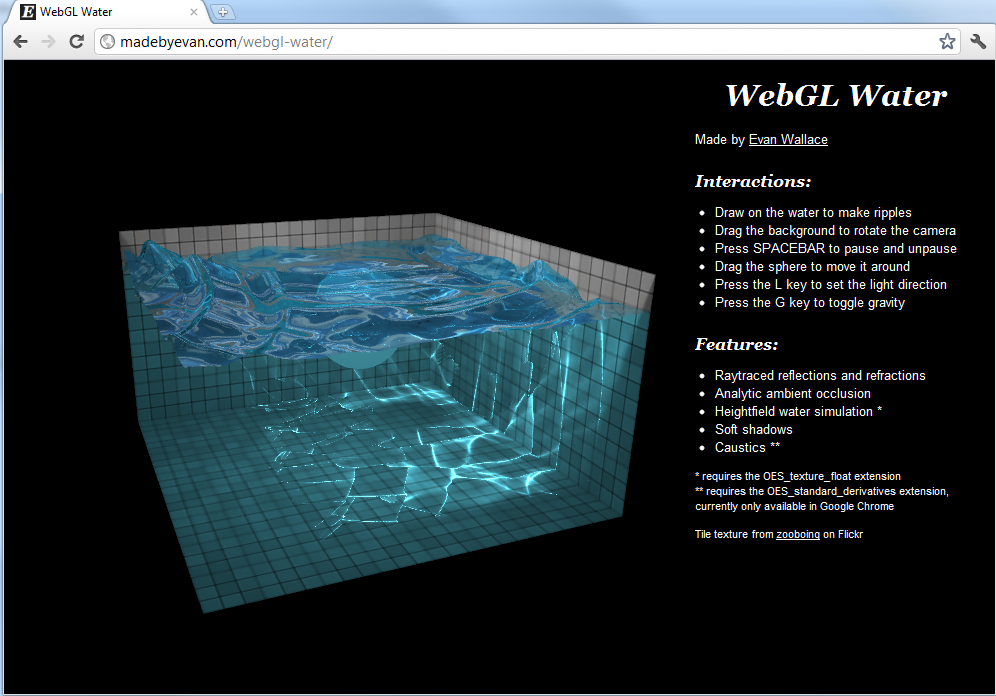
\includegraphics[height=\imgheight,width=\imgwidth]{webglwater}
  \caption{WebGL Water {--} Utilizando o processamento para obter
  bonitas cenas em 3D}
  \label{img:webglwater}
\end{figure}

Apesar de bonitos e interessantes, esses exemplos são apenas provas de
conceito para mostrar que o WebGL é realmente útil e pode ser
utilizado para aplicações que exigem um grande processamento do
navegador. Mas além de provas de conceito, alguns jogos já estão
utilizando WebGL como tecnologia auxiliar para acelerar no desenho dos
gráficos e nos cálculos.
Na Figura~\ref{img:emberwind} é possível ver um exemplo do jogo Emberwind
sendo executado utilizando WebGL.

\begin{figure}[H]
  \centering
	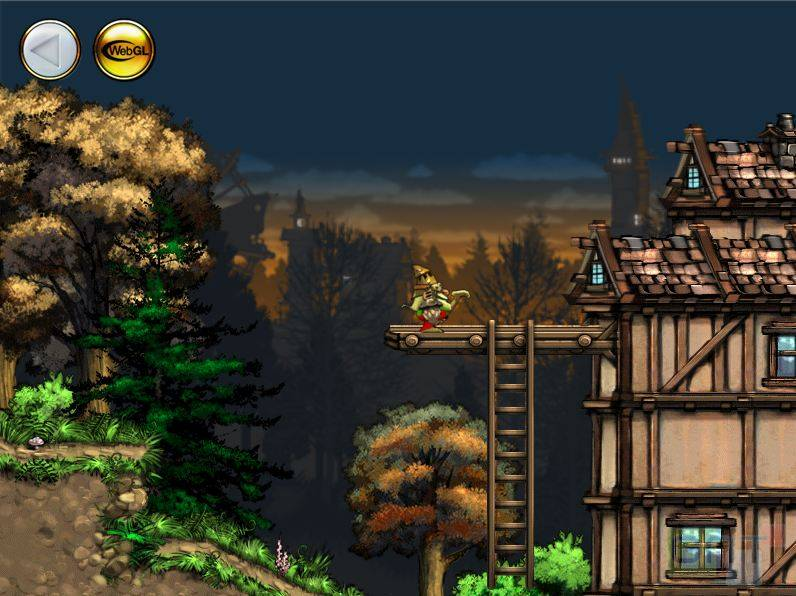
\includegraphics[height=\imgheight,width=\imgwidth]{emberwind}
  \caption{Emberwind {--} Utilizando o poder do WebGL para acelerar o processamento}
  \label{img:emberwind}
\end{figure}

Esse jogo em particular está sendo portado para a plataforma web,
fortificando o argumento dado neste subcapítulo. Uma particularidade
desse jogo é a opção de se utilizar apenas canvas para os dispositivos
que não suportam WebGL, o que mostra que é possível contornar a falta
de suporte do WebGL para jogos casuais nos dispositivos atuais, assim
como foi dito previamente.

\clearpage
